\documentclass[10pt]{beamer}
\usetheme{jambro}

\title[]{Matemática Aplicada - Apresentação}
\author[]{Paulo Victor da Fonseca}
\date{27 de fevereiro de 2023}

\hypersetup{
    colorlinks = true,
    urlcolor = teal,
    linkcolor = white    
}
\usepackage[portuguese]{babel}
\usepackage{subfig}
\usepackage{emoji}

\newtheorem{obj}{Objetivo}
\newtheorem{ementa}{Ementa}

\begin{document}

\begin{frame}[plain]
    \titlepage{
        \begin{center}
            \begin{minipage}{0.8\textwidth}
                \centering
            \end{minipage}
        \end{center}}
\end{frame}

\section{Docente}
\begin{frame}{Docente}
    \begin{tabular}{cl}
        \begin{tabular}{c}
            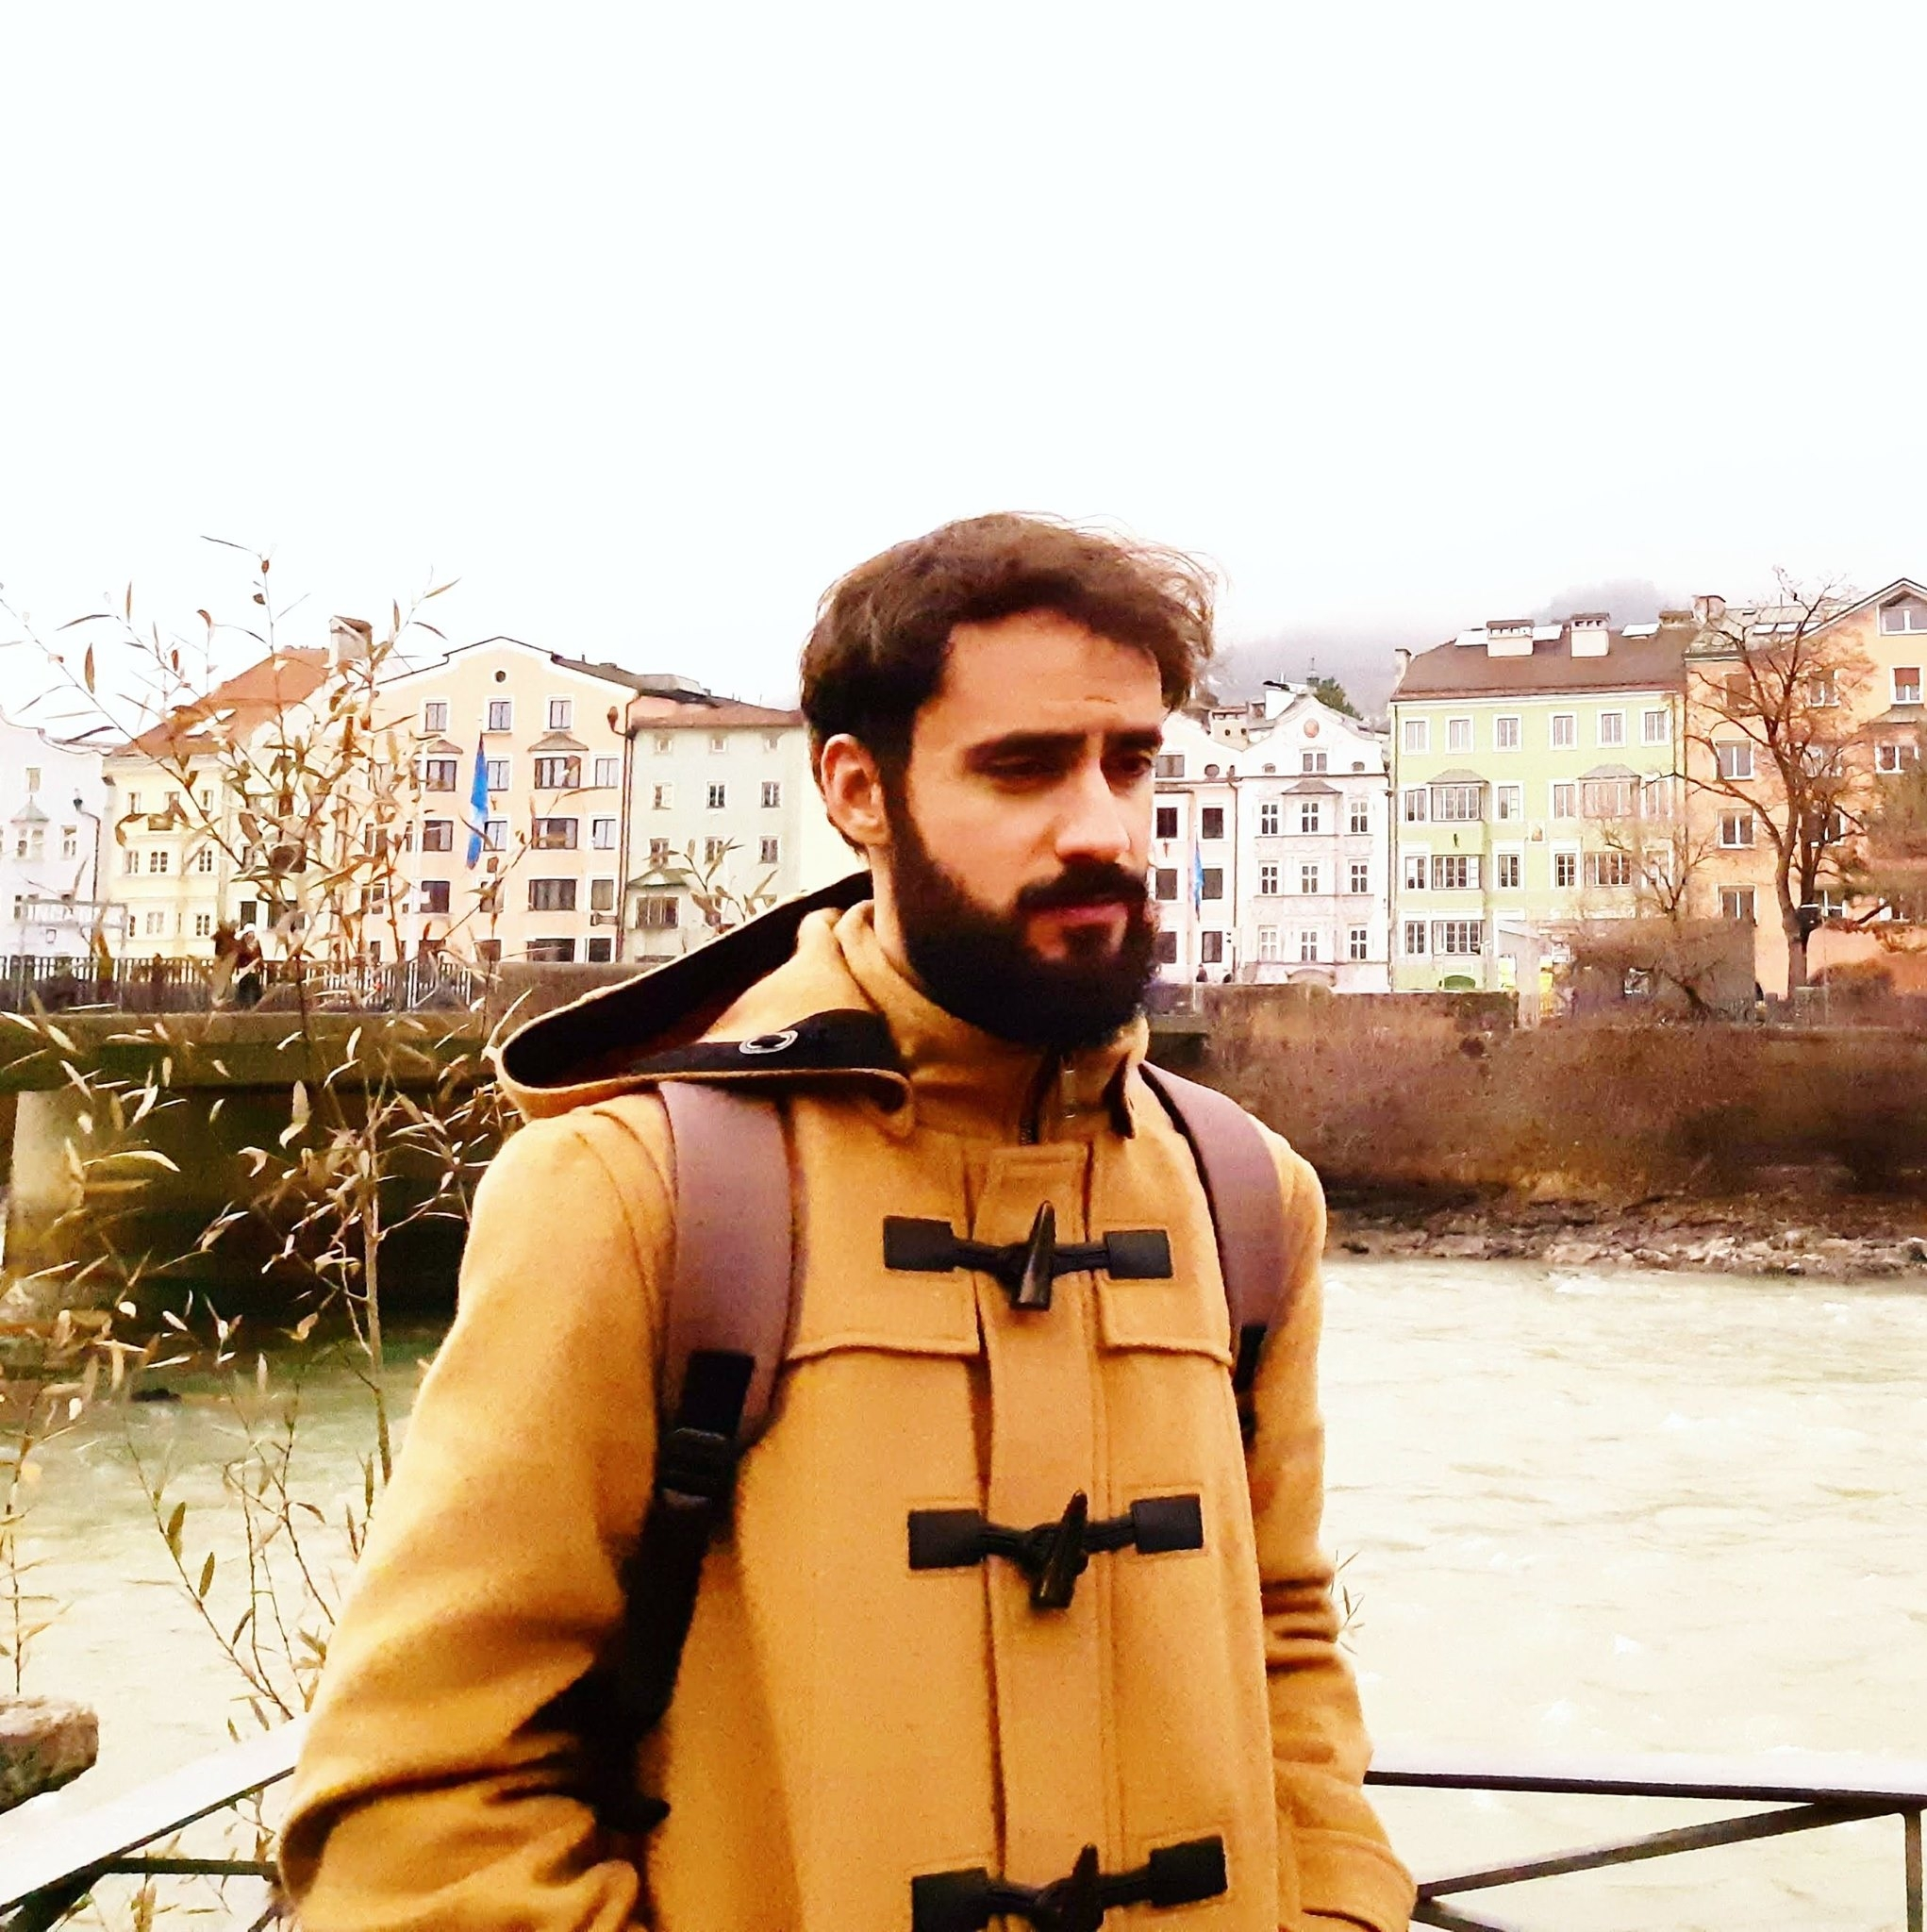
\includegraphics[width=3.5cm]{./figures/Paulo}
        \end{tabular}
         & \begin{tabular}{l}
               \parbox{0.6\linewidth}{%  change the parbox width as appropiate
                   \begin{itemize}
                    \item \textbf{Nome:} Paulo Victor da Fonseca\medskip
                    \item \textbf{Formação:} Doutorado em Economia - UFSC\medskip
                    \item \textbf{Áreas de pesquisa:} Macroeconomia. Políticas monetária e fiscal. Modelos DSGE. Modelos novo-Keynesianos com agentes heterogêneos. Modelos baseados em agentes.\medskip
                    \item \textbf{Website:} \href{https://pvfonseca.github.io}{pvfonseca.github.io}\medskip
                    \item \textbf{Contato:} \href{mailto:paulo.fonseca@udesc.br}{paulo.fonseca@udesc.br}
                \end{itemize}
               }
           \end{tabular} \\
    \end{tabular}
\end{frame}

\section{Ementa}
\begin{frame}{Matemática Aplicada: Ementa}
    \begin{center}
        \begin{minipage}{.9\textwidth}
            \NB{Conjuntos e funções (com ênfase em modelagem matemática aplicada a administração). Limite, continuidade, derivação e noções de integração. Sistemas de equações lineares e Matrizes. Aplicações computacionais.
            }
        \end{minipage}
    \end{center}

\end{frame}

\section{Objetivo}
\begin{frame}{Matemática Aplicada: objetivo}
    \begin{center}
        \begin{minipage}{.9\textwidth}
            \NB{O objetivo da disciplina é desenvolver o raciocínio e habilidade do aluno na utilização da linguagem matemática, através do estudo de cálculo diferencial e integral para funções univariadas e da resolução de sistemas de equações lineares.}
        \end{minipage}
    \end{center}

    O curso será dividido em quatro blocos:\medskip
    \begin{enumerate}
        \item Introdução e conceitos fundamentais\medskip

        \item Cálculo diferencial\medskip

        \item Cálculo integral\medskip

        \item Elementos de modelos lineares e álgebra linear
    \end{enumerate}
\end{frame}

\section{Formato das aulas e avaliações}
\begin{frame}{Formato das aulas e sistema de avaliação}
    \begin{itemize}
        \item A disciplina apoia-se, fundamentalmente, em livros-texto e notas de aula e será ministrada por meio de aulas expositivas.\bigskip

        \item As aulas acontecerão às:
              \begin{itemize}
                  \item Segundas-feiras das 18:50 às 20:30
                  \item Quartas-feiras das 20:45 às 22:25\bigskip
              \end{itemize}

        \item A avaliação será realizada a partir dos procedimentos abaixo:
              \begin{itemize}
                  \item Atividade avaliativa I (PI): 20\%
                  \item Atividade avaliativa II (PII): 30\%
                  \item Atividade avaliativa III (PIII): 30\%
                  \item Trabalhos adicionais: 20\%\bigskip
              \end{itemize}

        \item Página da disciplina no GitHub: \href{https://github.com/pvfonseca/mtm\_aplicada}{github.com/pvfonseca/mtm\_aplicada}
    \end{itemize}
\end{frame}

\begin{frame}{Formato das aulas e sistema de avaliação}
    \begin{itemize}
        \item Os alunos devem ter em mente que o aprendizado e o acompanhamento do curso dependem essencialmente de seu próprio esforço.\bigskip

        \item Os tópicos do programa serão apresentados em aulas expositivas, destinadas à apresentação de conceitos, modelos e suas aplicações.\bigskip

        \item[\emoji{warning}] \hlight{Embora importantes, as aulas n\~{a}o podem jamais ser vistas como substitutas da leitura regular e cuidadosa dos textos indicados e da resolu\c{c}\~{a}o dos exerc\'{i}cios propostos.}
    \end{itemize}

\end{frame}
\section{Bibliografia}

\begin{frame}{Bibliografia \emoji{books}}
    \begin{figure}
        \centering
        \subfloat[Stewart (2016)\label{fig1a}]{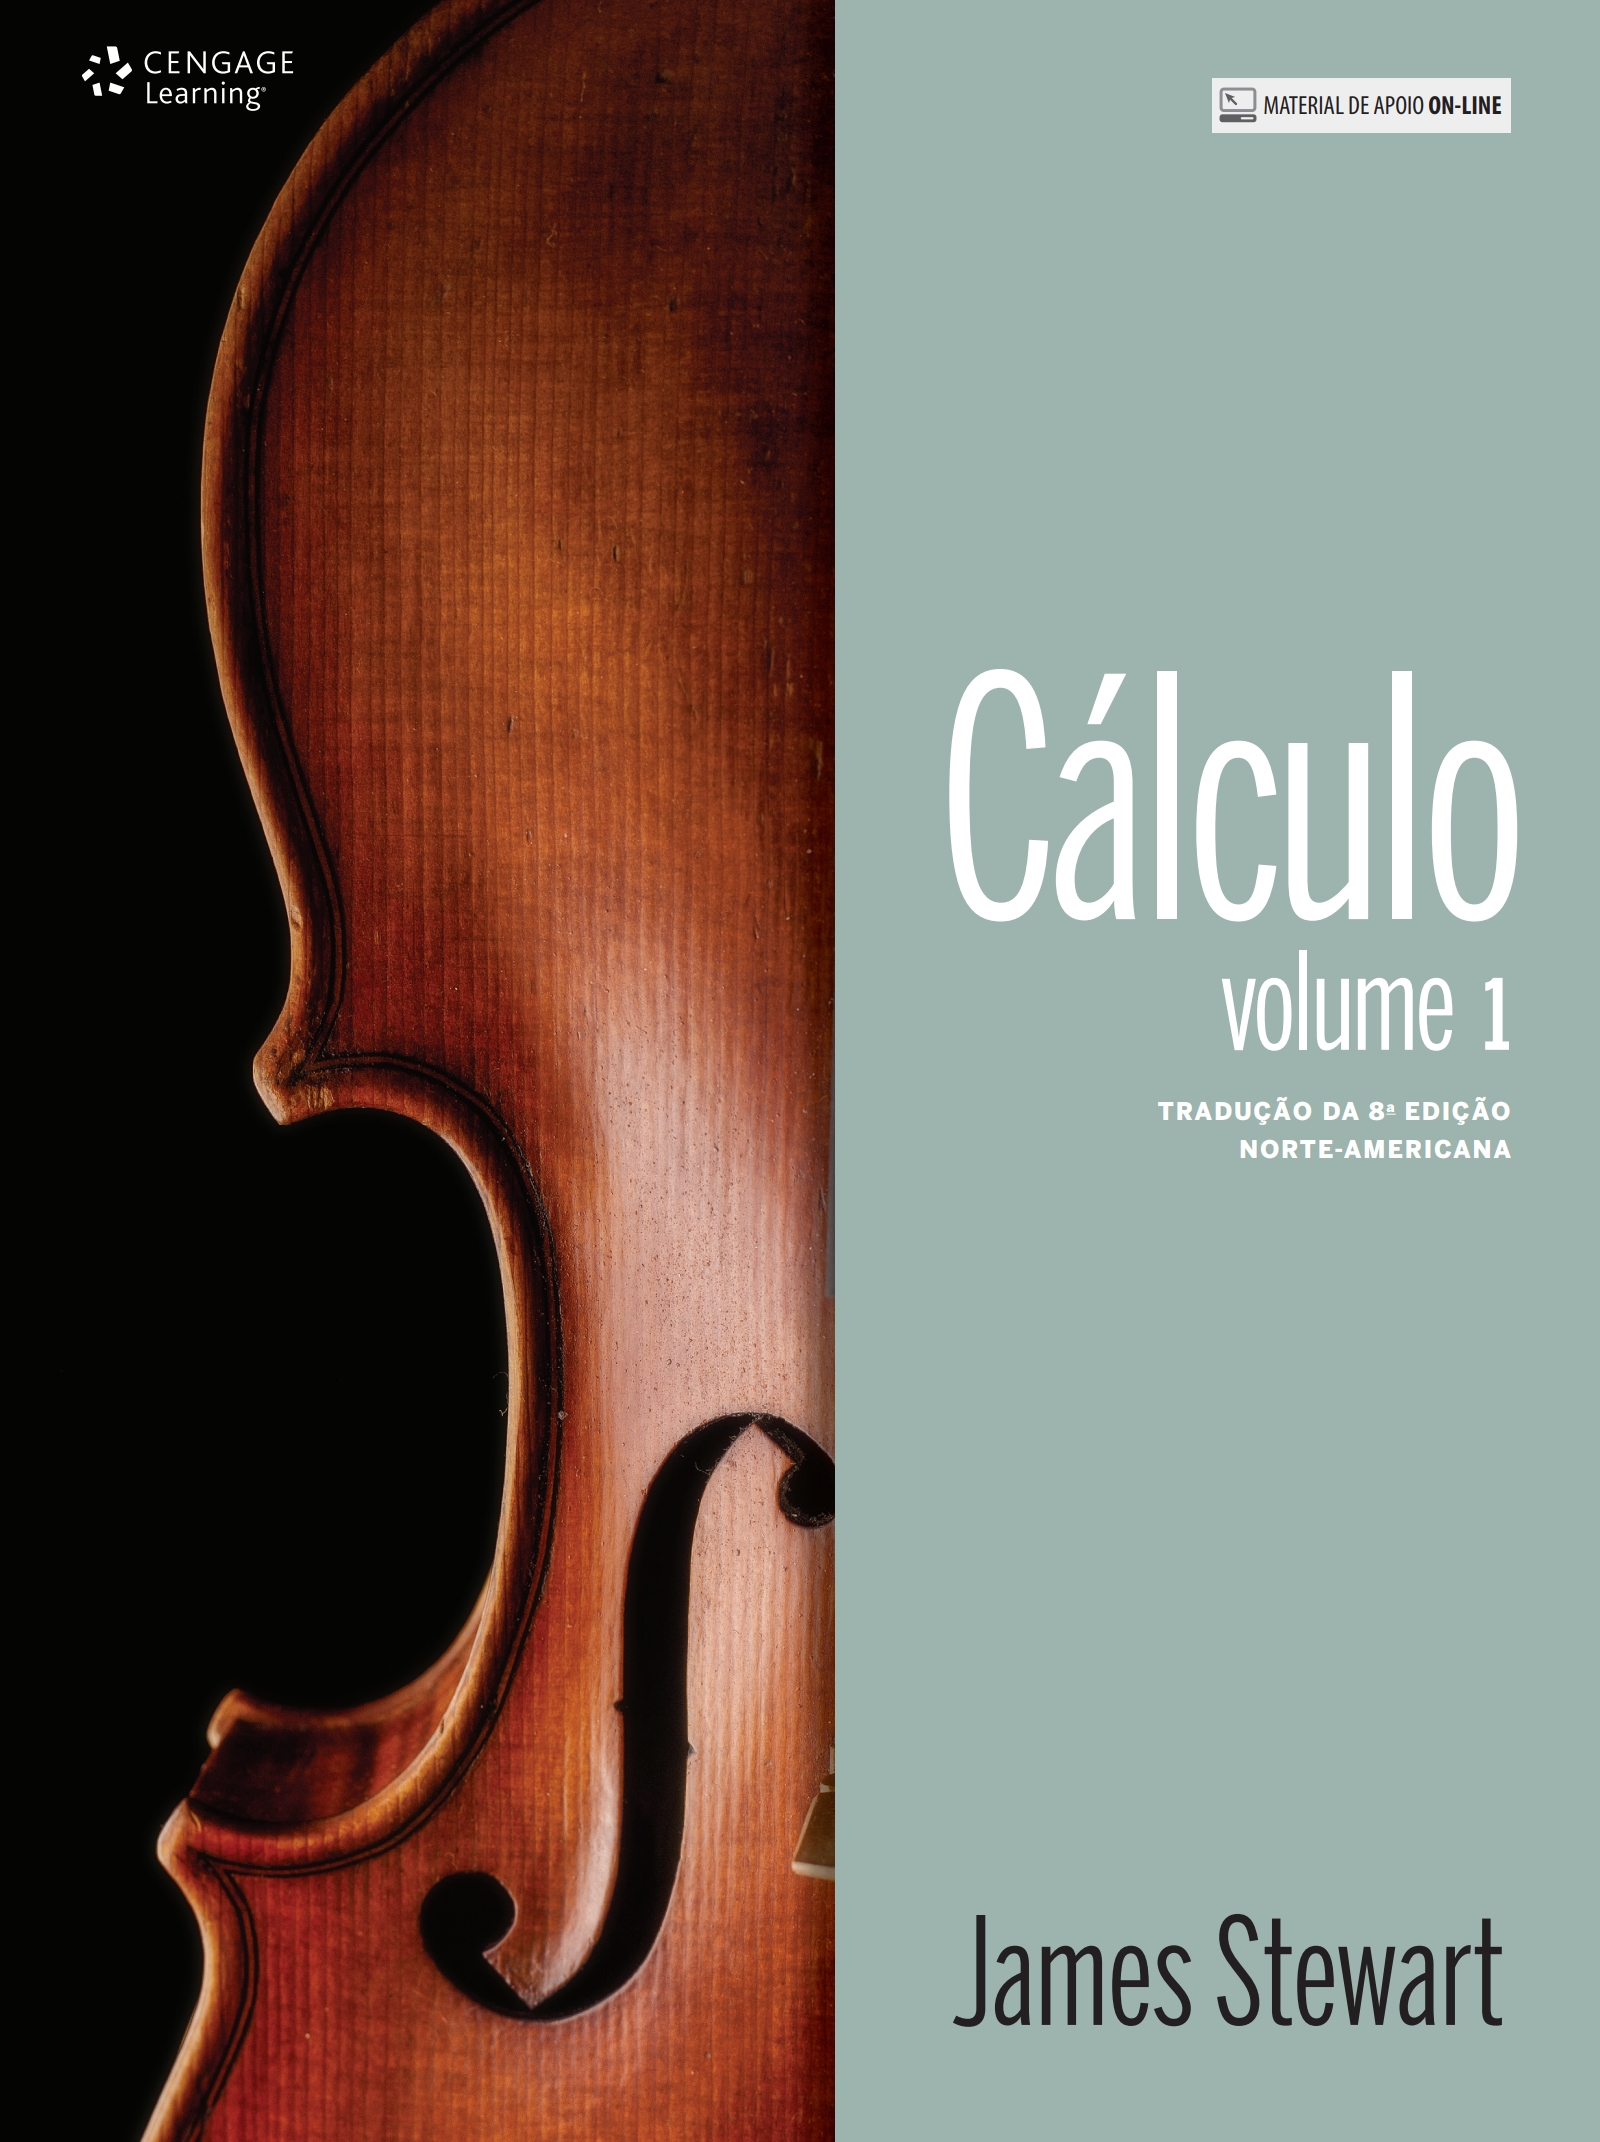
\includegraphics[width=0.25\textwidth]{./figures/stewart}} \quad
        \subfloat[Strang (2009)\label{fig1b}]{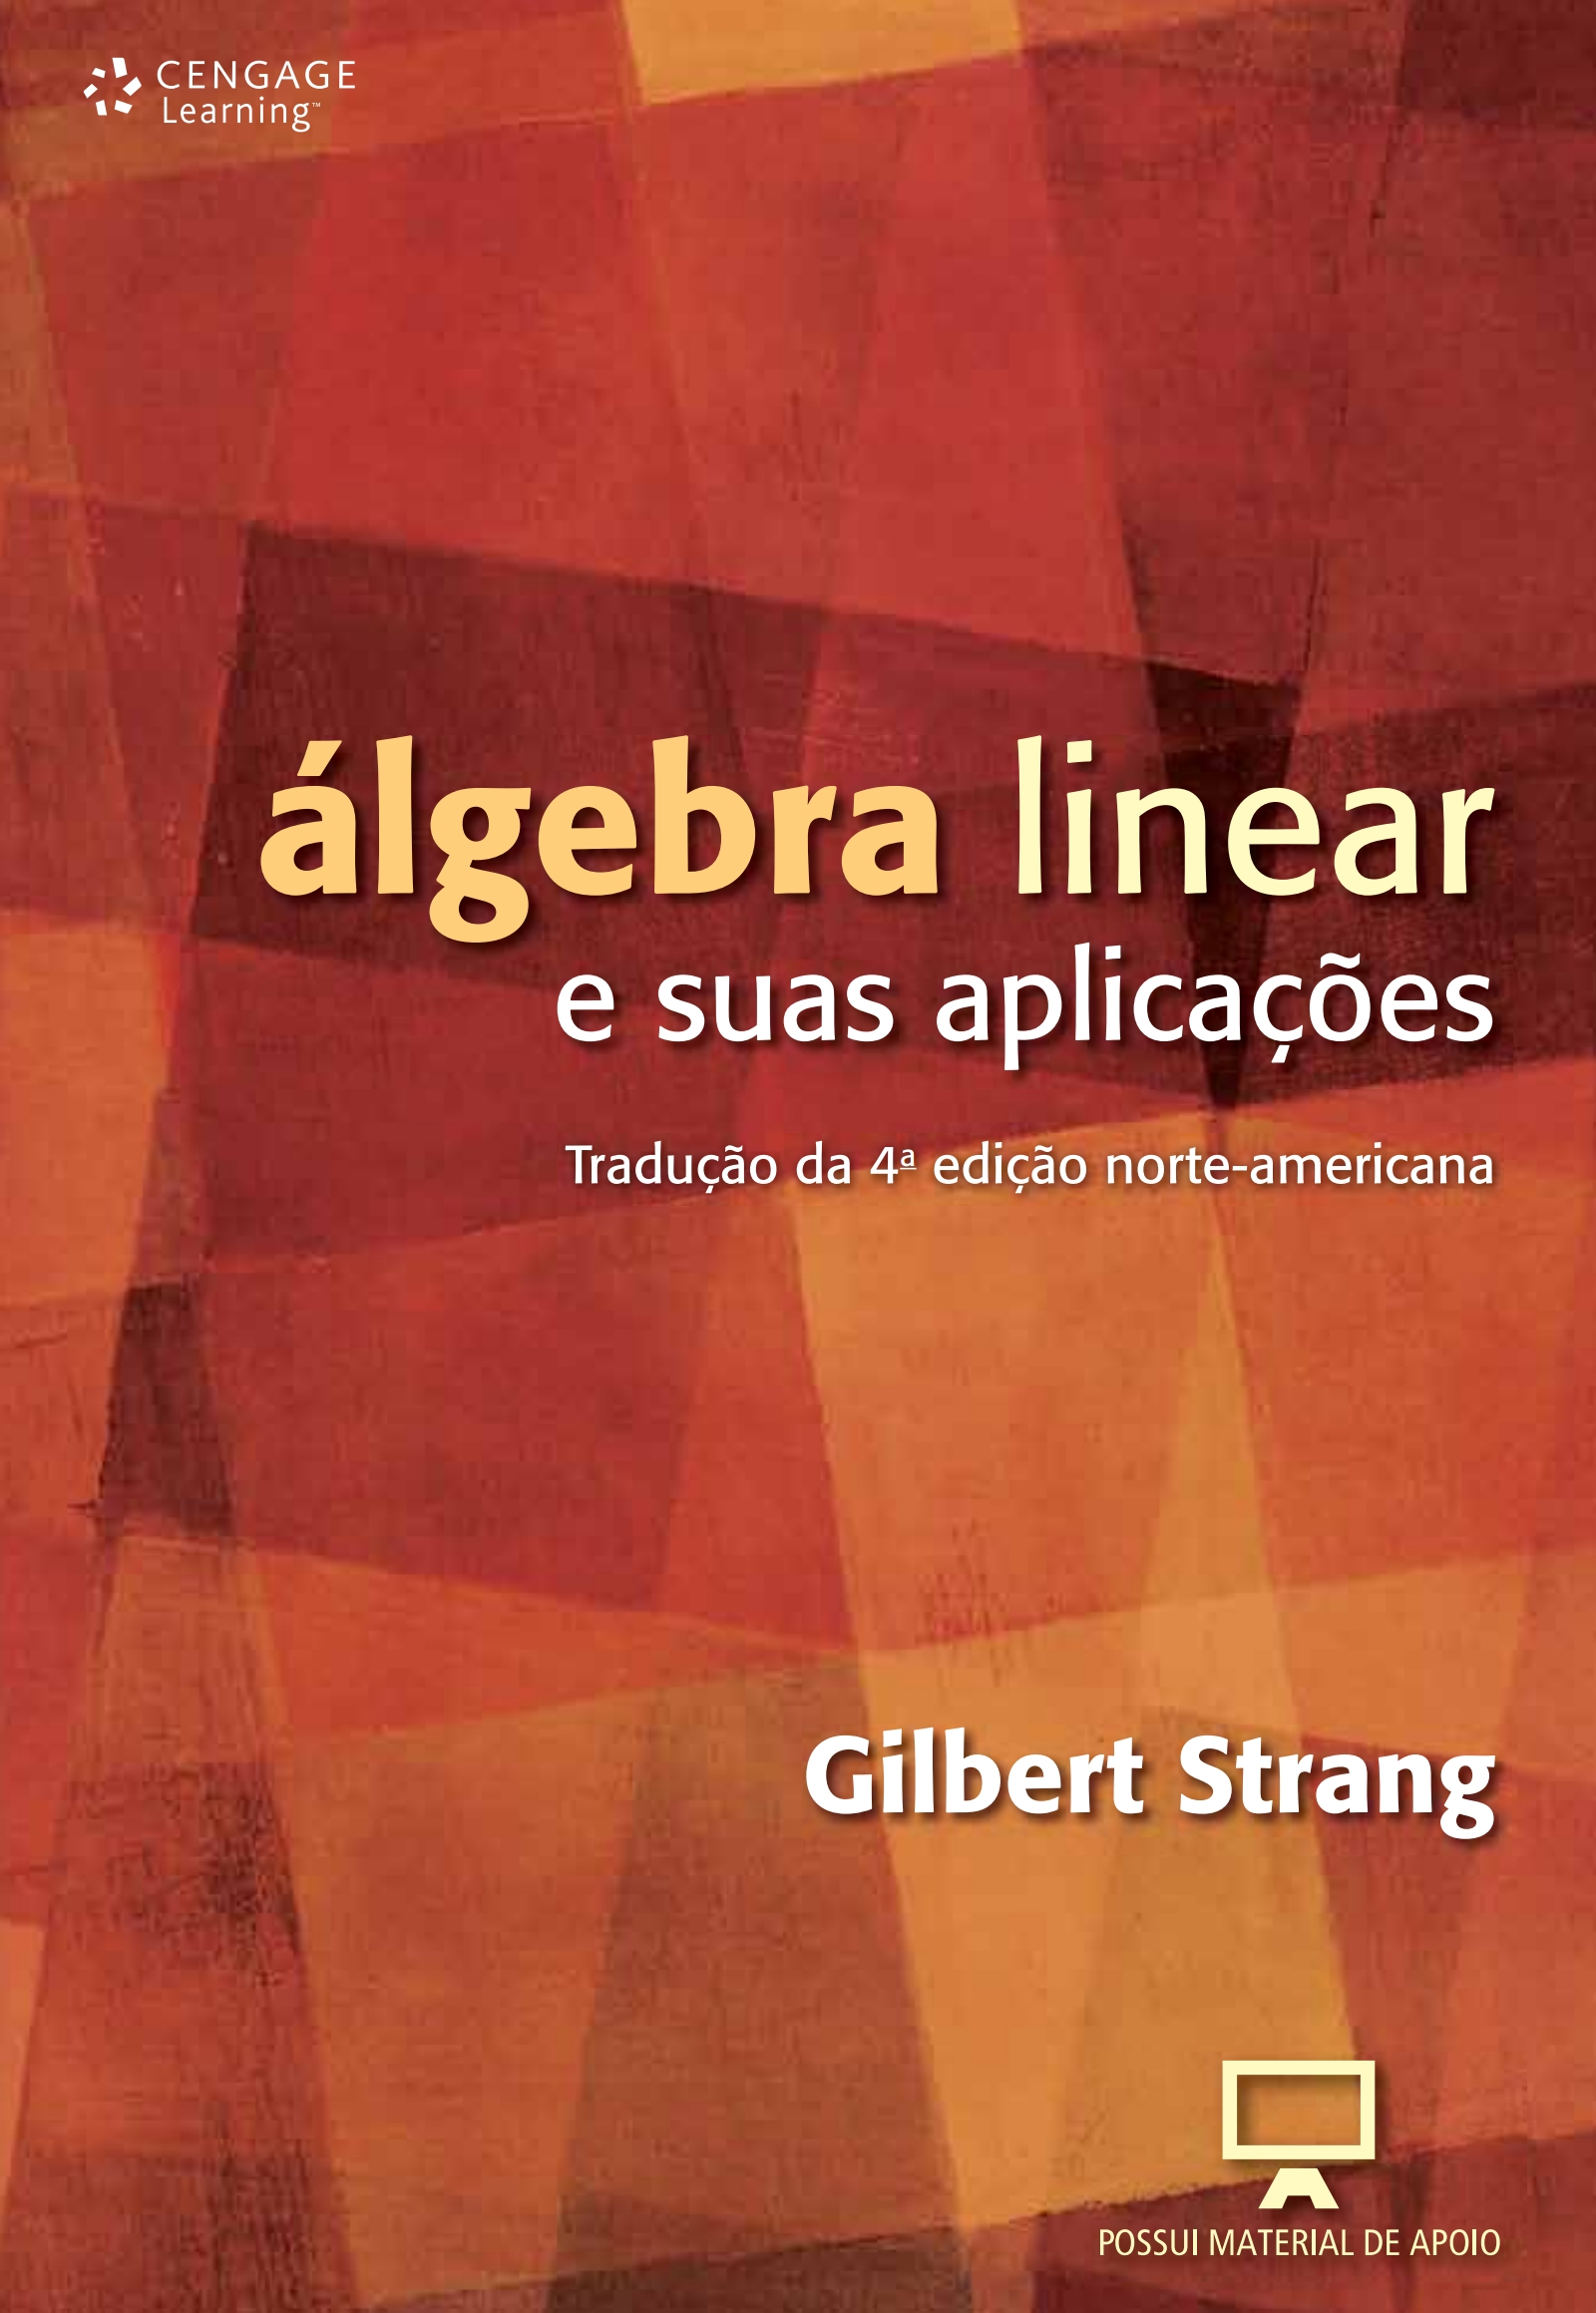
\includegraphics[width=0.25\textwidth]{./figures/strang}} \quad
        \subfloat[Spivak (2006)\label{fig1c}]{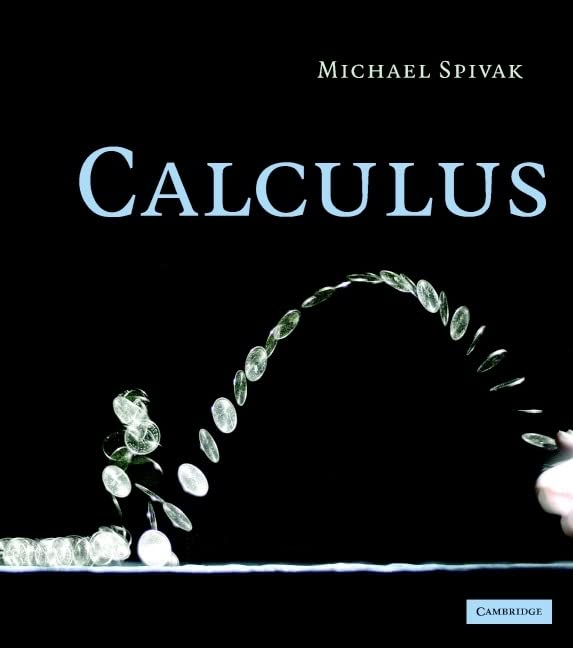
\includegraphics[width=0.25\textwidth]{./figures/spivak}}
        \caption{Bibliografia do curso}
        \label{fig1}
    \end{figure}
\end{frame}

\begin{frame}{Bibliografia \emoji{books}}
    \begin{figure}
        \centering
        \subfloat[Guidorizzi (2010)\label{fig2a}]{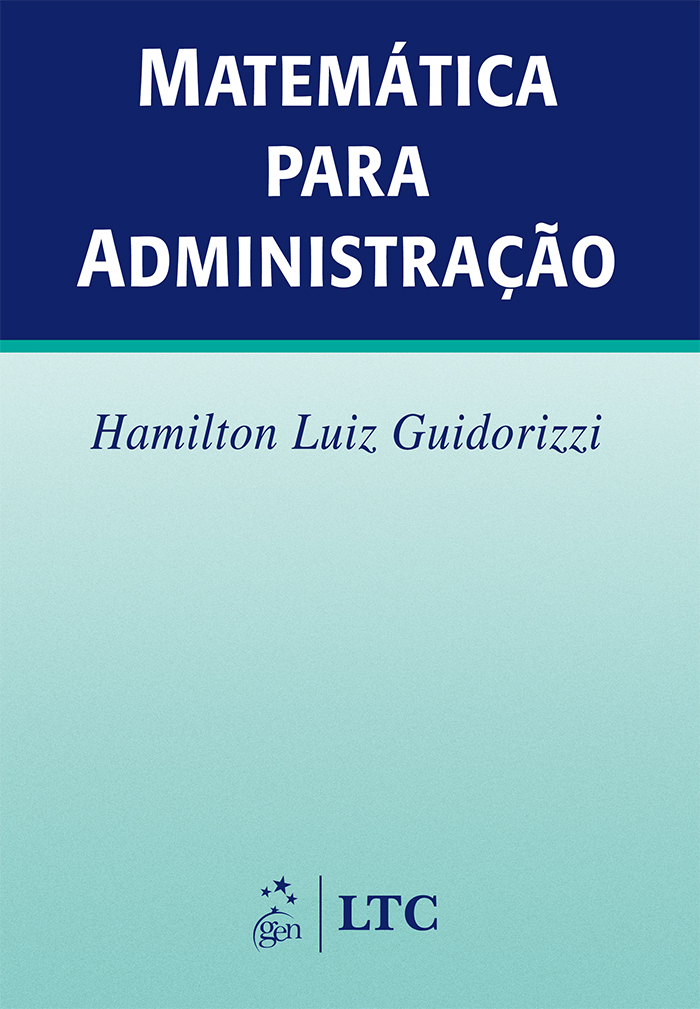
\includegraphics[width=0.2\textwidth]{./figures/guidorizzi}} \quad
        \subfloat[Leite (2015)\label{fig2b}]{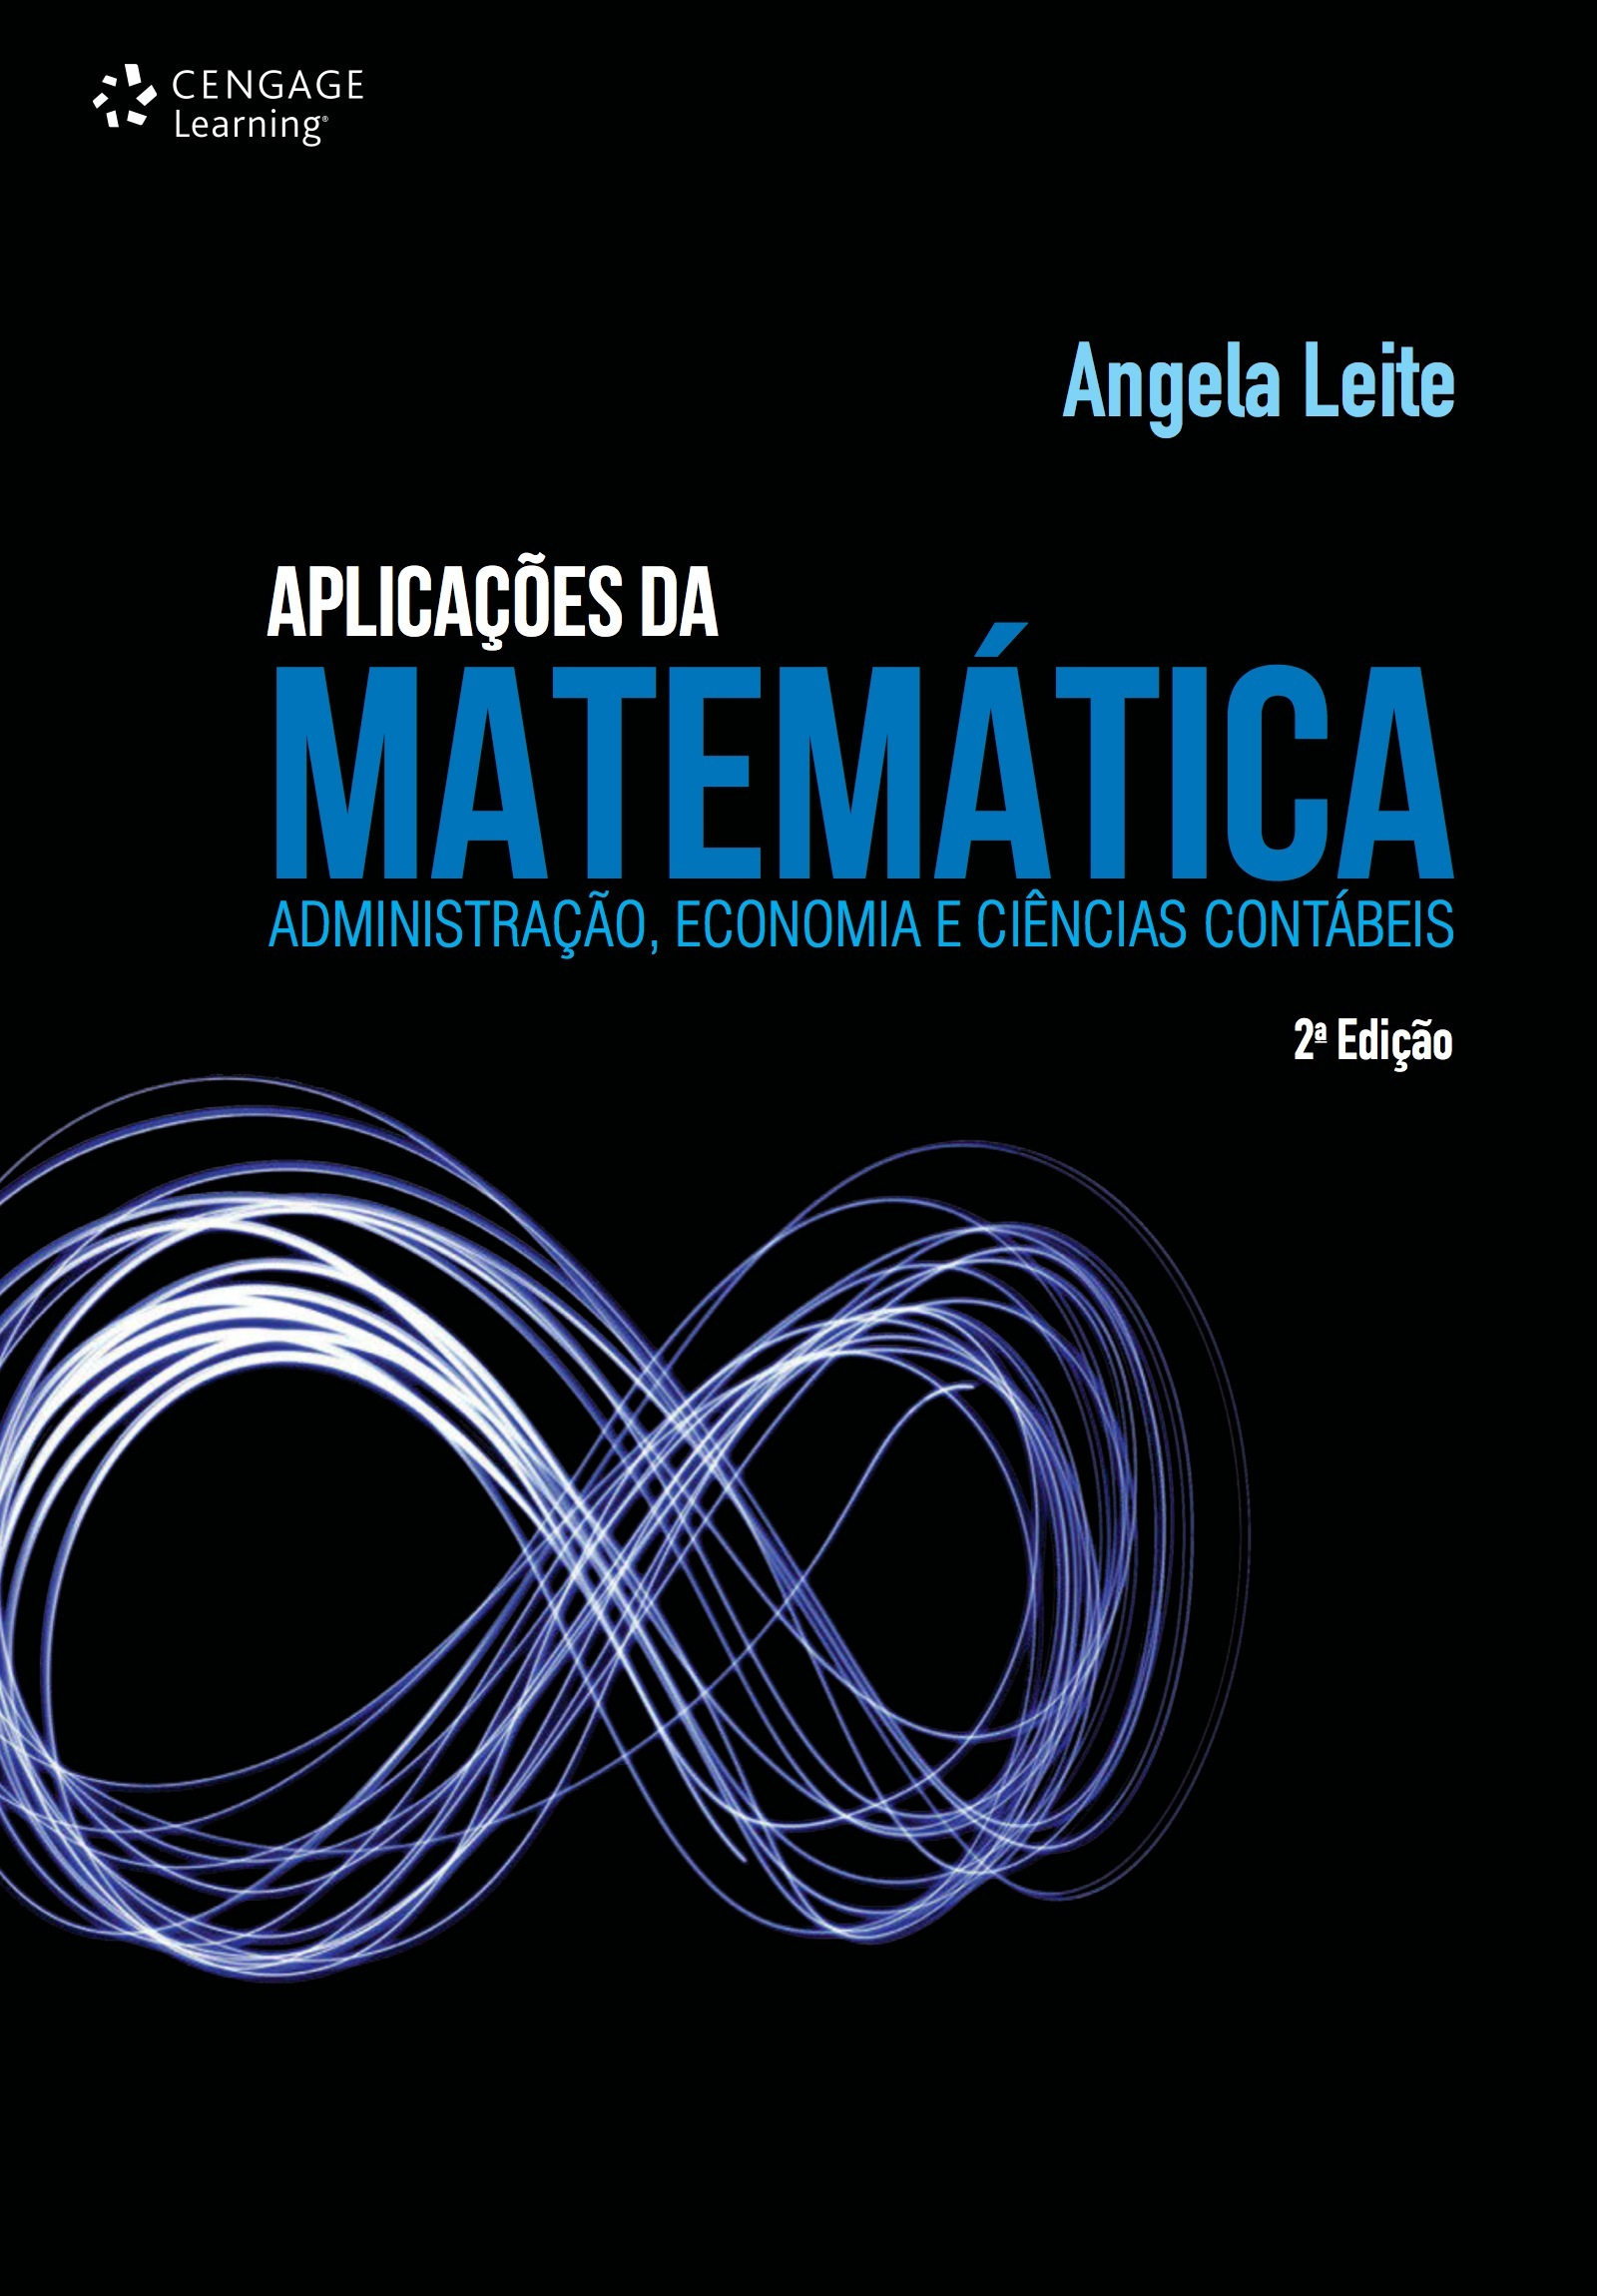
\includegraphics[width=0.2\textwidth]{./figures/leite.jpg}}  \quad
        \subfloat[Murolo e Bonetto (2012)\label{fig2c}]{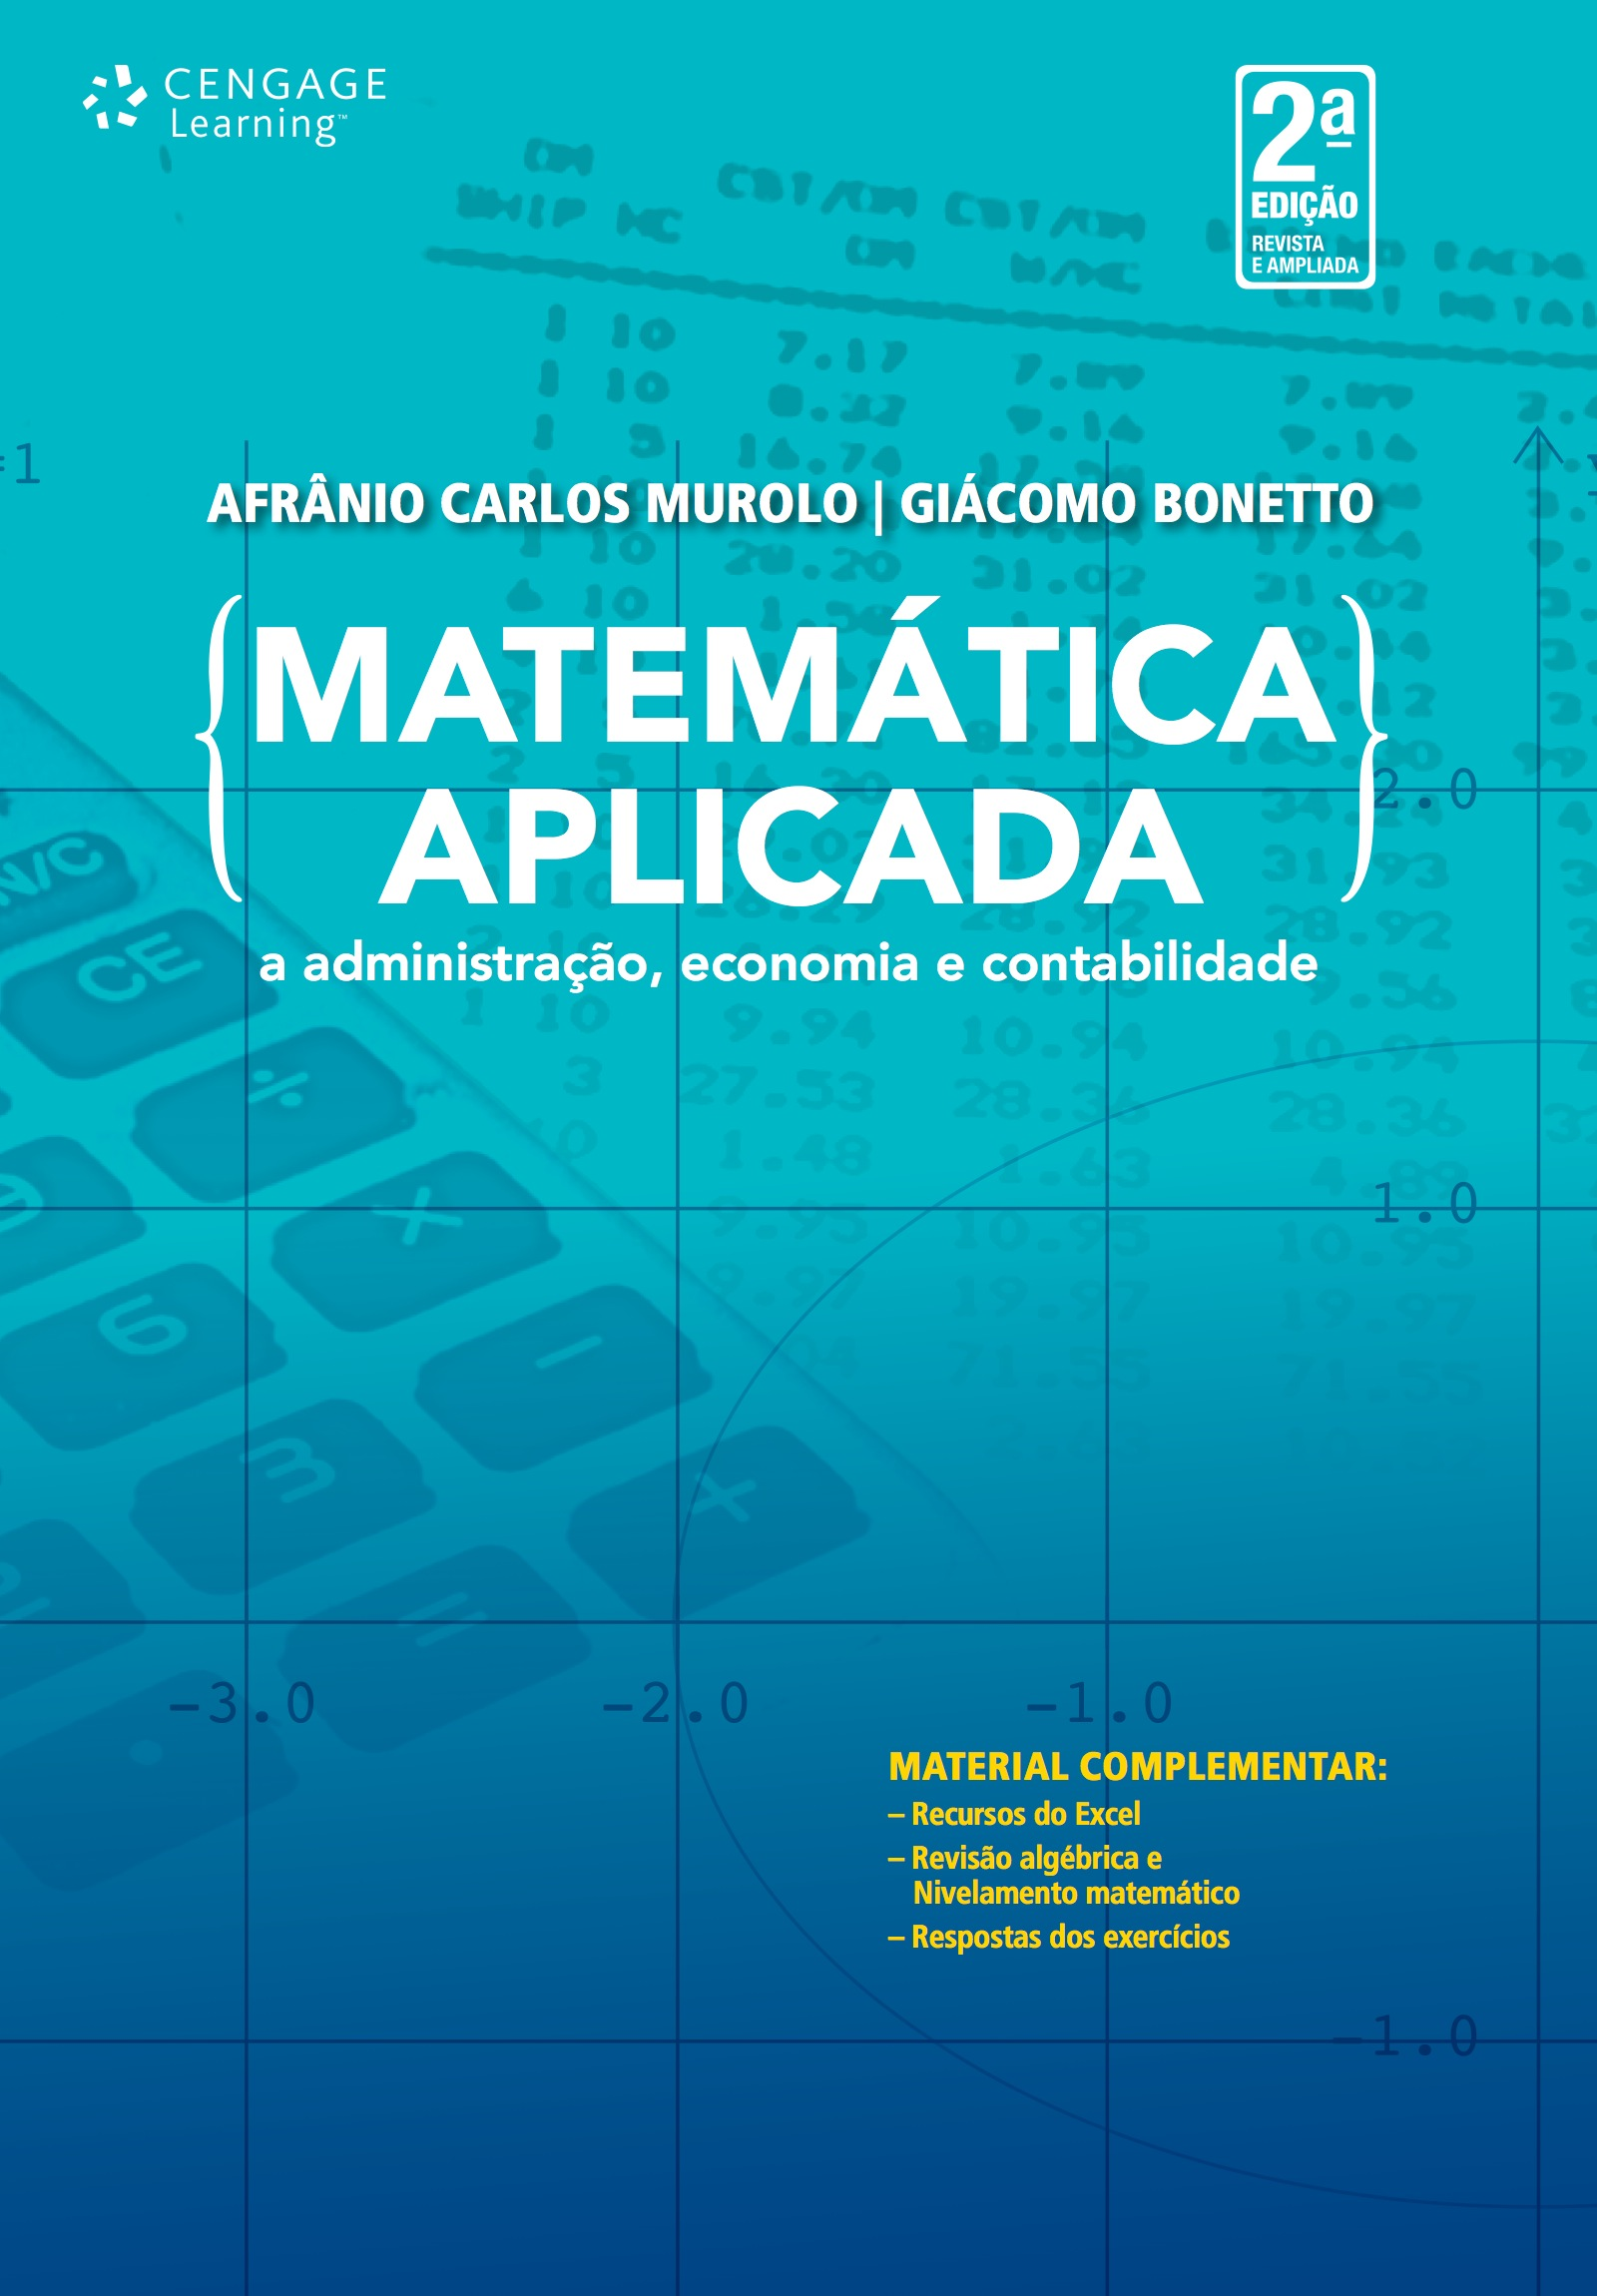
\includegraphics[width=0.2\textwidth]{./figures/murolo}} \quad
        \subfloat[Silva e Machado (2014)\label{fig2d}]{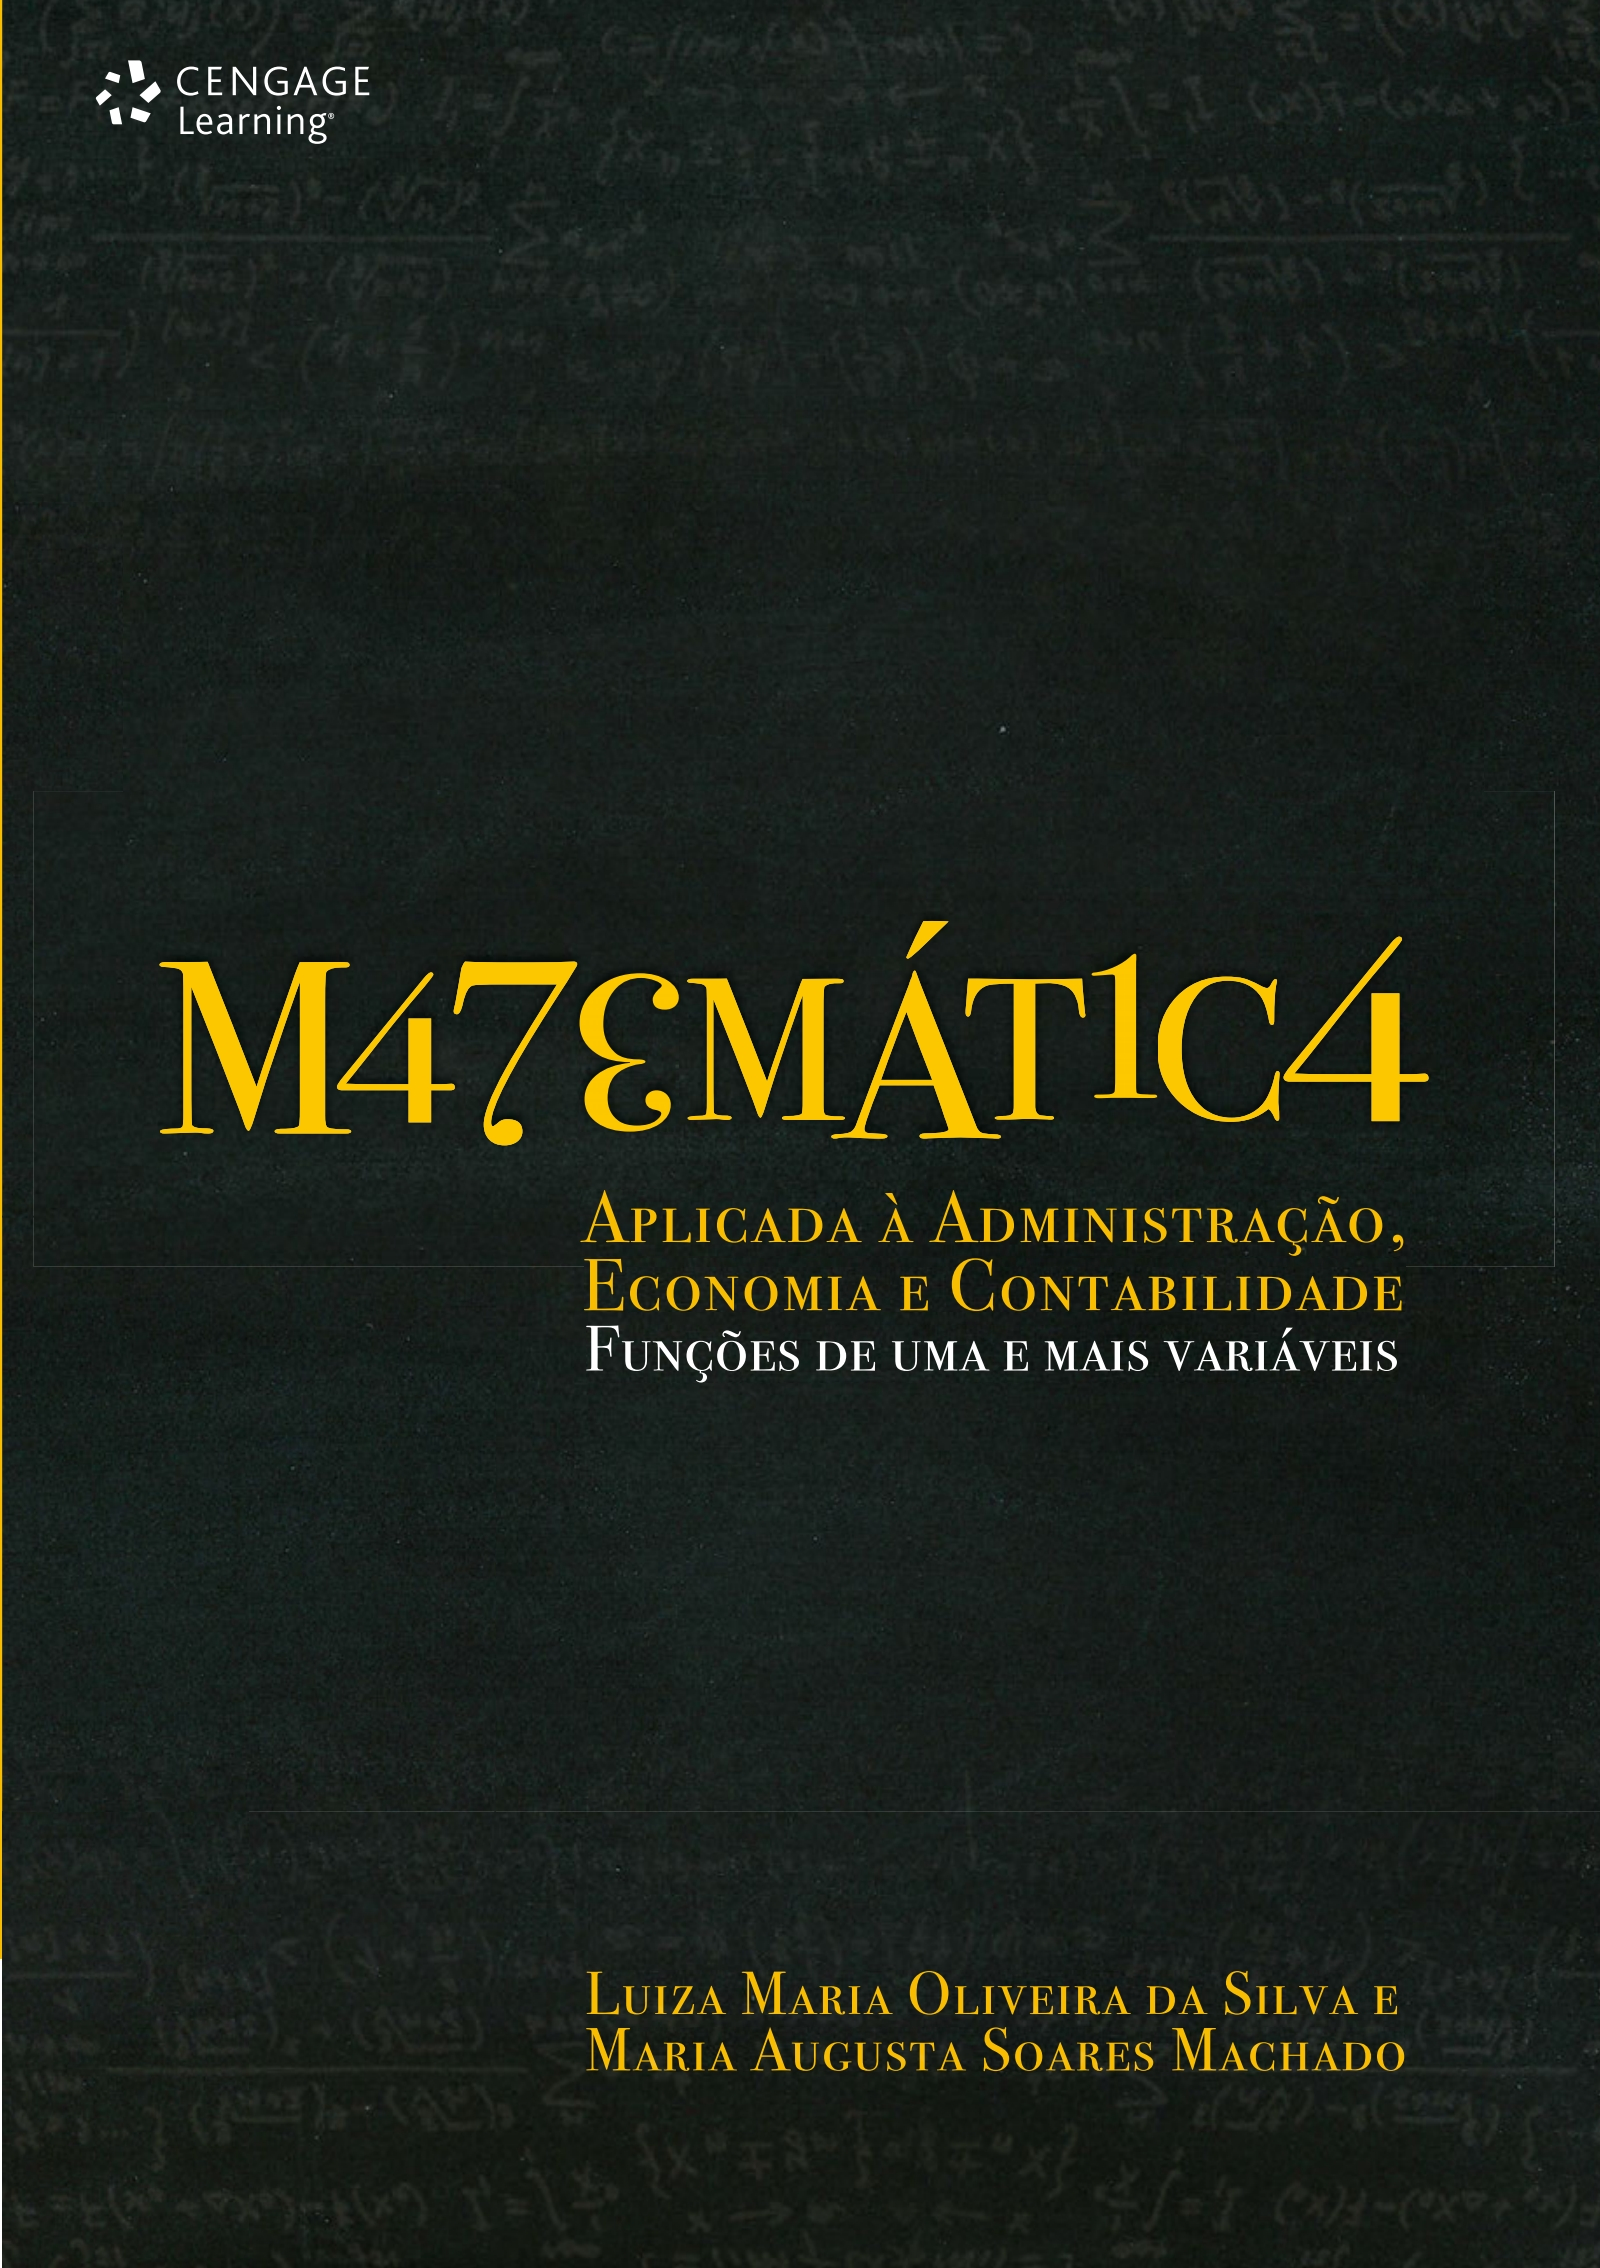
\includegraphics[width=0.2\textwidth]{./figures/silva}}
        \caption{Bibliografia do curso}
        \label{fig2}
    \end{figure}
\end{frame}

\begin{frame}{Bibliografia \emoji{books}}
    \begin{itemize}
        \item GUIDORIZZI, H.L. \href{https://app.minhabiblioteca.com.br/reader/books/978-85-216-2778-4}{Matemática para administração}. Rio de Janeiro: LTC, 2010.
        \item LEITE, A. \href{https://app.minhabiblioteca.com.br/reader/books/9788522122707}{Aplicações da matemática: administração, economia e ciências contábeis}. 2.ed. São Paulo: Cengage Learning, 2015.
        \item MUROLO, A.C; BONETTO, G. \href{https://app.minhabiblioteca.com.br/reader/books/9788522113392}{Matemática aplicada à administração, economia e contabilidade}. 2.ed. São Paulo: Cengage Learning, 2012. % Disponível em: app.minhabiblioteca.com.br/reader/books/9788522113392
        \item SILVA, L.M.O; MACHADO, M.A.S. \href{https://app.minhabiblioteca.com.br/reader/books/9788522126576}{Matemática aplicada à administração, economia e contabilidade: funções de uma e mais variáveis}. São Paulo: Cengage Learning, 2014. % Disponível em: app.minhabiblioteca.com.br/reader/books/9788522126576
        \item SPIVAK, M. Calculus. 3.ed. Cambridge University Press, 2006.
        \item STEWART, J. \href{https://app.minhabiblioteca.com.br/reader/books/9788522126859}{Cálculo: volume I}. 8.ed. São Paulo: Cengage Learning, 2016. % Disponível em: app.minhabiblioteca.com.br/reader/books/9788522126859
        \item STRANG, G. \href{https://app.minhabiblioteca.com.br/reader/books/9788522118021}{Álgebra linear e suas aplicações}. 4.ed. São Paulo: Cengage Learning, 2009. \bigskip % Disponível em: app.minhabiblioteca.com.br/reader/books/9788522118021
    \end{itemize}
    \emoji{warning} Bibliografias adicionais poderão ser indicadas no decorrer da disciplina.
\end{frame}
\end{document}